\documentclass{article}

% Packages
\usepackage[a4paper, left=2.0cm, right=2.0cm, top=2.0cm, bottom=2.0cm]{geometry}
\usepackage{longtable,booktabs} % For tables
\usepackage{caption} % Customisable captions
\usepackage{graphicx} % Required for including pictures
\usepackage{authblk} % For formatting authors
\usepackage{amsmath} % For maths typesetting
\usepackage{lineno} % Add line numbers with \linenumbers
\usepackage[toc,page]{appendix} % For formatting/numbering appendix
\usepackage[utf8]{inputenc} % For UTF8 character encoding
\usepackage{url}
\usepackage{microtype}
\usepackage{parskip}
\usepackage[super]{natbib} % References
\usepackage{makecell} % For line breaks in a table
\usepackage{subcaption} % Allows use of subfigures
\usepackage{lmodern} % A scalable font - avoids erros due to non-sclabale fonts
\usepackage{lipsum} % For generating test text
\usepackage{multicol}
\usepackage{tabularx} % To allow tables to be full page width
\DeclareUnicodeCharacter{2060}{\nolinebreak} % Prevent unicode (U+2060) error on local complile
\usepackage{afterpage} % For palcing tabel at top of next page
\let\endtitlepage\relax % Avoid page break after title page

% New commands for maths symbols:
\newcommand{\mRS}{\rm{mRS}} % mRS for math mode
\newcommand{\tne}{\ensuremath{t_\mathrm{ne}}} % Time-of-no-effect

\newcommand{\logodds}{log(odds)} % log odds for normal text
\newcommand{\logoddsratio}{log(odds ratio)} % log odds for normal text

% Extra commands for draft only: 
%\usepackage{ulem} % for strikeout \sout
% Make commands for fancy notes

% Have different references in Appendix
\usepackage{multibib}
\newcites{appendix}{References for Appendix}
% https://www.overleaf.com/learn/latex/Using_colours_in_LaTeX#Named_colours_provided_by_the_xcolor_package
\usepackage[usenames,dvipsnames,svgnames,table]{xcolor}
\newcommand{\Anna}[1]{\textcolor{Green}{#1}}
% pick a different colour if you prefer:
\newcommand{\Kerry}[1]{\textcolor{Purple}{#1}}
\newcommand{\Mike}[1]{\textcolor{Teal}{#1}}
\newcommand{\checkthis}[1]{\textcolor{Orange}{#1}}






\begin{document}

% Info on wordcounts:
% https://www.overleaf.com/learn/how-to/Is_there_a_way_to_run_a_word_count_that_doesn%27t_include_LaTeX_commands%3F

% To include refs in word count:
%TC:incbib

% Ignore title and abstract in word count
%TC:ignore

% Add line numbers if needed
% \linenumbers

% Title page
\title{Modelling disability-level and utility outcome in stroke patients depending on time to intravenous thrombolysis and mechanical thrombectomy. Application to England and Wales.\\}

\author[1, 2]{Anna Laws}
\author[1, 2]{*Michael Allen}
\author[1, 2]{Kerry Pearn}
\author[3]{Peter McMeekin}
\author[4, 2]{Martin James}

\affil[1]{\footnotesize University of Exeter Medical School.}
\affil[2]{\footnotesize NIHR South West Peninsula Applied Research Collaboration (ARC).}
\affil[3]{\footnotesize Department of Nursing, Midwifery \& Health, Northumbria University}
\affil[4]{\footnotesize Royal Devon University Healthcare NHS Foundation Trust}
\affil[*]{\footnotesize Corresponding author: m.allen@exeter.ac.uk}
\maketitle

% Sections
\section*{Abstract} % Use * to avoid numbering section

Write abstract here!

%TC:endignore


\begin{multicols}{2}
\section{Introduction}

% Have 5 paragraphs:
% 1. Background - stroke and benefit of IVT & MT
% 2. Problem being addressed: planning services and benefit of IVT and MT under different service models
% 3. What do we know: dichotomised outcome models
% 4. What don't we know: more detailed models on mRS, shift, Utility
% 5. What does this work seek to address and how


% 1. Background - stroke and benefit of IVT & MT

Globally, stroke presents a very significant, and growing, health burden. In 2019, stroke was the second-leading cause of death (11·6\% of total deaths) and the third-leading cause of death and disability combined (5·7\% of total disability-adjusted life years) \cite{feigin_global_2021}. For ischaemic strokes, the cause of the majority of strokes, the disabling effect may be reduced by reperfusion treatment with intravenous thrombolysis (IVT) \cite{emberson_effect_2014} or mechanical thrombectomy (MT) \cite{fransen_time_2016, goyal_endovascular_2016}, with both treatments reducing in effectiveness within hours of stroke onset.

% 2. Problem being addressed: planning services and benefit of IVT and MT under different service models

When considering acute treatment options, ischaemic stroke may be divided into two broad categories: non-large vessel (nLVO) occlusions may be treated with IVT, and large vessel occlusions (LVO) may be treated with IVT and MT. IVT is a medical treatmentment that may be broadly provided in acute stroke units. Provision of MT is a more specialist service requiring expert interventional radiologists providing procedures in a specialist Computed Tomography (CT) lab. For LVO, MT adds significant clinical benefit over IVT alone \cite{fransen_time_2016, goyal_endovascular_2016}. As both IVT and MT are time-dependent, the optimal organisation of acute stroke services requires careful thought; IVT may most rapidly be provided by a patient attending their closest IVT unit. MT may most rapidly be provided by a patient attending their closest MT unit, but this may require them travelling further than their closest IVT unit, thus delaying IVT for the sake of faster MT. Optimal provision of acute stroke services requires consideration of how to balance time to IVT and MT, which will inform ambulances on where it is best to take any individual patient when there is a choice of a closer IVT-only unit, or a more distant MT-capable unit.

% 3. What do we know
As time to both IVT and MT important, but there may be a choice minimising time to IVT or MT, modelling has been used extensively to help predict the outcome of different models of emergency stroke care. For example, Holodinsky and co-workers have modelled the trade-off between time to IVT both as a general model \cite{holodinsky_drip-and-ship_2018} and applied to specific geographies \cite{kamal_geographic_2018}. These models are probabilistic models predicting a dichotomous outcome of either good or bad outcomes of achieving a certain disability threshold, depending on time to treatment. Schlemm and co-workers have extended this type of model to predict changes in disability-adjusted life years, depending on the probability of re-canalisation with IVT and MT given at different times \cite {schlemm_comparative_2019}. Venema and colleagues presented a stroke outcome model that predicts disability-level outcome, depending on time to MT and IVT \cite{venema_personalized_2019}. That particular model was an advancement on previous models, but was limited by the clinical data available and used, such as assuming that the clinical trials on thrombolysis were treating nLVO only, and by a lack of published information of pre-stroke mRS levels of the stroke patient population, which presents the 'best case' improvement in outcome.

% 4. What don't we know: more detailed models on mRS, shift, Utility.  5. What does this work seek to address and how
The work described here seeks to extend, and build on, the above mentioned work in two key ways: 1) We seek to use the latest and most comprehensive data available to produce disability-level outcome models of reperfusion treatment in stroke, and 2) we aim to produce a model with a primary aim of being able to be reproduced by others, using both detailed descriptions of all assumptions and calculations, and parallel publication of code (using Python, a free and open source computer programming language).
\end{multicols} % Use 'input' rather than 'include' to avoid page breaks
\section{Methods}

\subsection{Modified Rankin Scale}

Modified Rankin Scale (mRS) is the most commonly used instrument to describe post-stroke functional outcome \cite{quinn_functional_2009}. Table \ref{tab:mrs} shows a description of the seven levels of mRS along with utilties, from Wang \emph{et al.}\cite{wang_utility-weighted_2020}. Utilities are a measure of the preference or value that an individual or society gives a particular health state, with 1 being full health and 0 being dead (values of less than zero describe states where death is considered preferable).

\begin{minipage}{\textwidth}
\renewcommand*{\arraystretch}{2.0} % adjust row spacing
\begin{longtable}[]{@{}llr@{}}
\caption{A description of modified Rankin Scale score, with Utilities from Wang \emph{et al.}\cite{wang_utility-weighted_2020}}\\
\toprule
mRS & Description. & Utility\tabularnewline
\midrule
\endhead
0 & No symptoms. & 0.97\tabularnewline
1 & No significant disability: Able to carry out all usual activities,
despite some symptoms. & 0.88\tabularnewline
2 & \makecell[l]{Slight disability: Able to look after own affairs without assistance, but unable to carry \\ out all previous activities.} &
0.74\tabularnewline
3 & Moderate disability: Requires some help, but able to walk
unassisted. & 0.55\tabularnewline
4 & \makecell[l]{Moderately severe disability: Unable to attend to own bodily needs without assistance, \\ and unable to walk unassisted.} & 0.20\tabularnewline
5 & Severe disability: Requires constant nursing care and attention,
bedridden, incontinent. & -0.19\tabularnewline
6 & Dead. & 0.00\tabularnewline
\bottomrule
\label{tab:mrs}
\end{longtable}
\end{minipage}

\subsection{Methods overview}

This model contains mRS outcome distributions for three patient-treatment cohorts

\begin{enumerate}
    \item nLVO treated with IVT
    \item LVO treated with IVT
    \item LVO treted with MT
\end{enumerate}

For each patient-treatment cohort, we estimate two mRS distributions: one mRS distribution if treatment is given at \emph{t = 0} (time of stroke onset), and one mRS distribution if treatment is given at \emph{t = No Effect} (time of no effect). In order to estimate these two mRS distributions, we use data from reperfusion treatment clinical trials and stroke admission data from England and Wales. To select the relevant patients for each cohort we will use the National Institutes of Health Stroke Scale (NIHSS) on arrival as a surrogate to classify patients as nLVO (NIHSS 0-10) or LVO (NIHSS 11+). NIHSS has been shown to have higher accuracy, in separating nLVO and LVO, than other stroke scales (Area under Receiver Operating Characteristic Curve = 0.86 \cite{duvekot_comparison_2021}).

All mRS distributions created are based on the assumption that, following treatment, the mRS distribution will lie between two extremes: 1) reperfusion perfectly restores function, and the resulting mRS distribution is the same as the pre-stroke mRS distribution (this data is obtained from Sentinel Stroke National Audit Programme, SSNAP, using 246,676 emergency stroke admissions to acute stroke teams in England and Wales between 2016 and 2018), and 2) reperfusion treatment fails to restore any function and the resulting mRS distribution is the same as a control untreated population. Both distributions are corrected for excess deaths that may be caused by the treatment (from clinical trials). To create required mRS distributions we find a weighting between these two extremes that give us a distribution that matches published reference points.

The \emph{t = 0} mRS distributions are calculated to give the expected mRS distributions if treatment was given immediately after stroke onset, and also include the risk of excess deaths caused by taking the treatment. Further details specific to stroke type and treatment type are given below.

The \emph{t = No Effect} mRS distributions are based on mRS distribution data when patients did not receive any treatment (this represents what will happen if the patient takes the treatment at \emph{t = No Effect}). This data is obtained from the untreated control group in clinical trials and further adjusted to include the risk of excess deaths caused by taking the treatment. Further details specific to stroke type and treatment type are given below.

To predict the effect of treatment at any given time, we assume that the log odds of being in any particular mRS category will vary linearly over time between \emph{t = 0} and \emph{t = No Effect} mRS distributions. This form of decay was fitted to clinical trial data for IVT \cite{emberson_effect_2014} and MT \cite{fransen_time_2016}. 
\section{results}


\begin{figure}
\centering
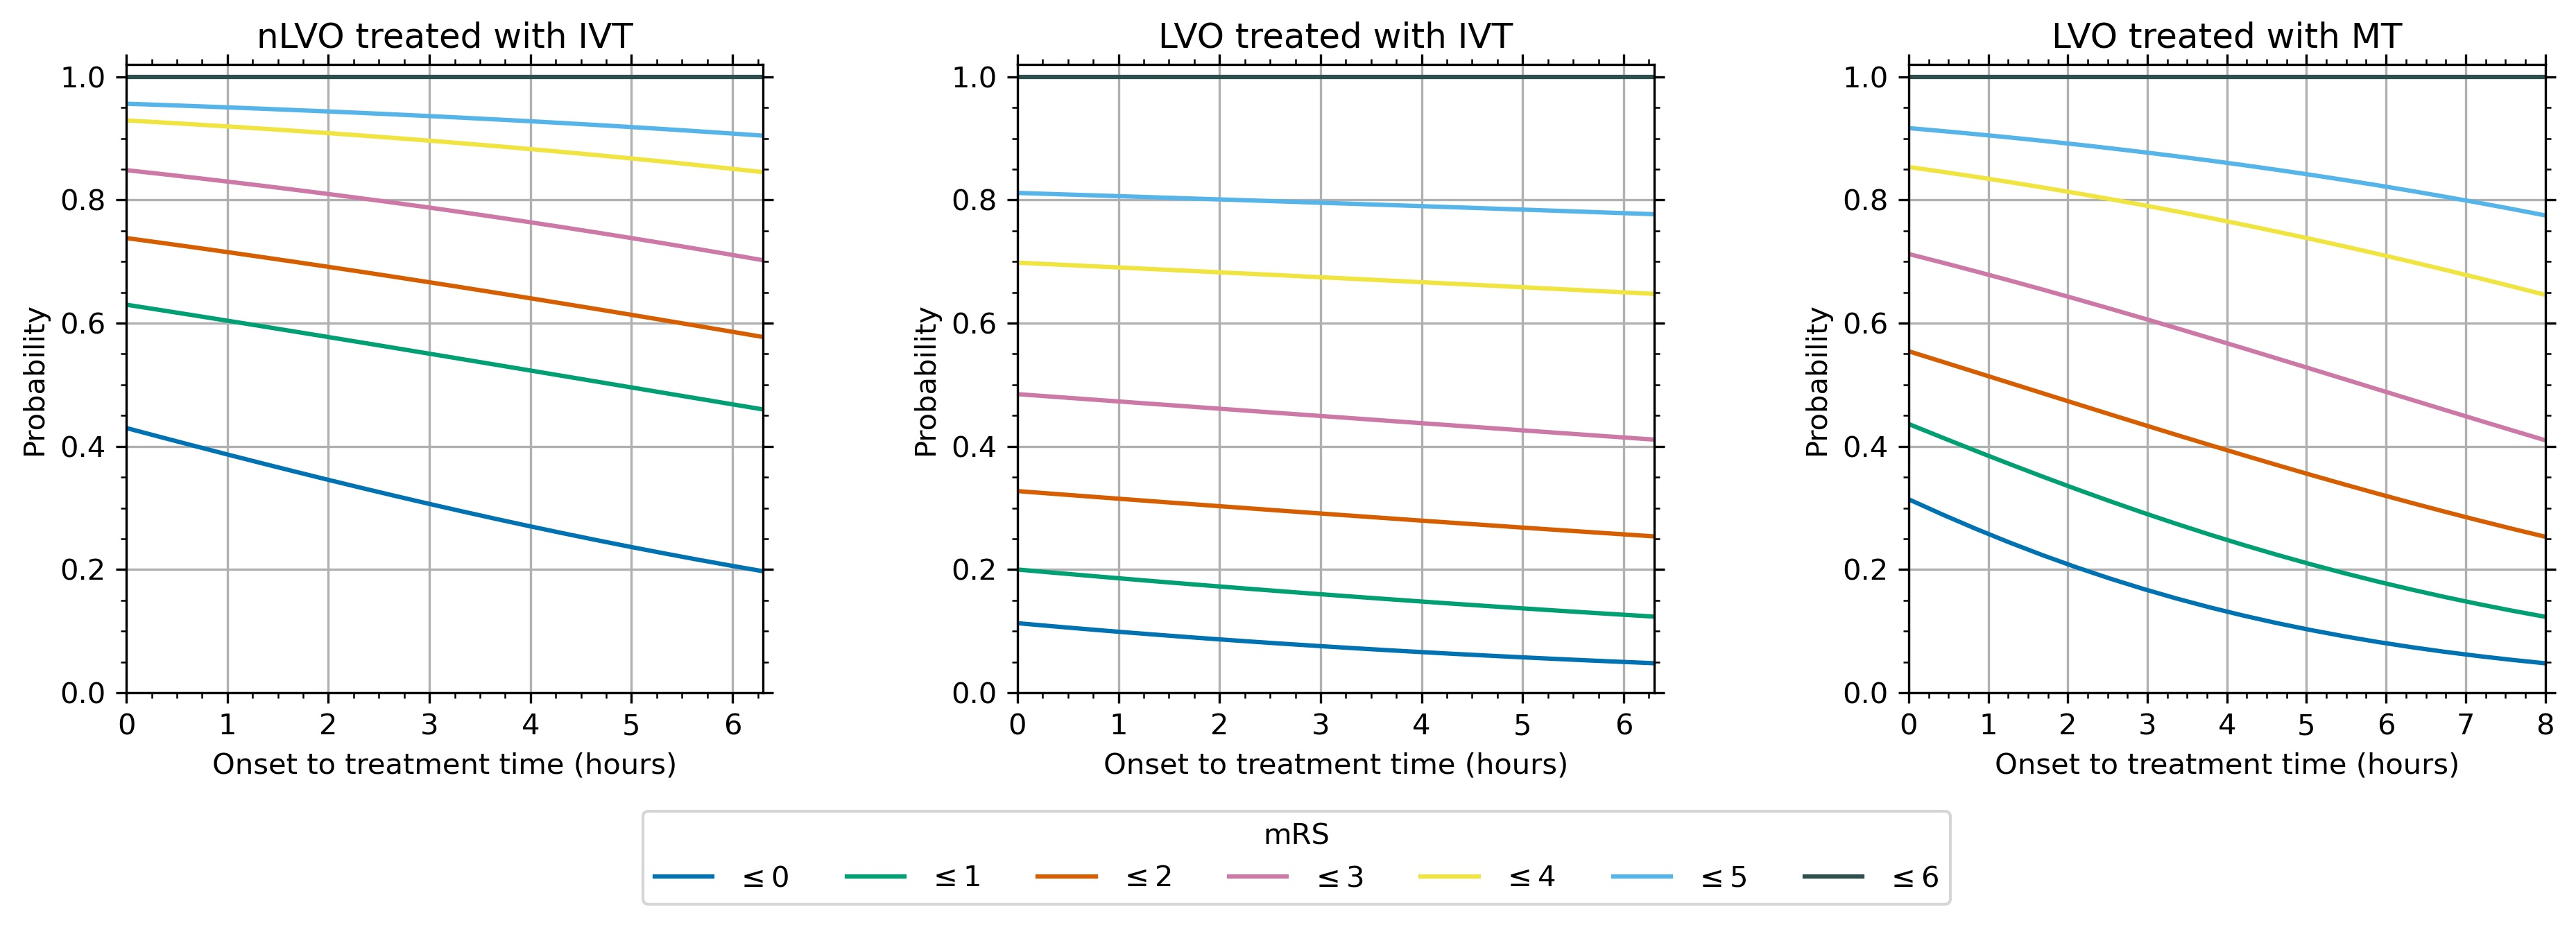
\includegraphics[width=1.0\textwidth]{./images/probs_with_time}
\caption{mRS probability distributions by time from onset to treatment. Left: nLVO treated with IVT. Middle: LVO treated with IVT. Right: LVO treated with MT.}
\label{fig:probs_with_time}
\end{figure}


\begin{figure}
\centering
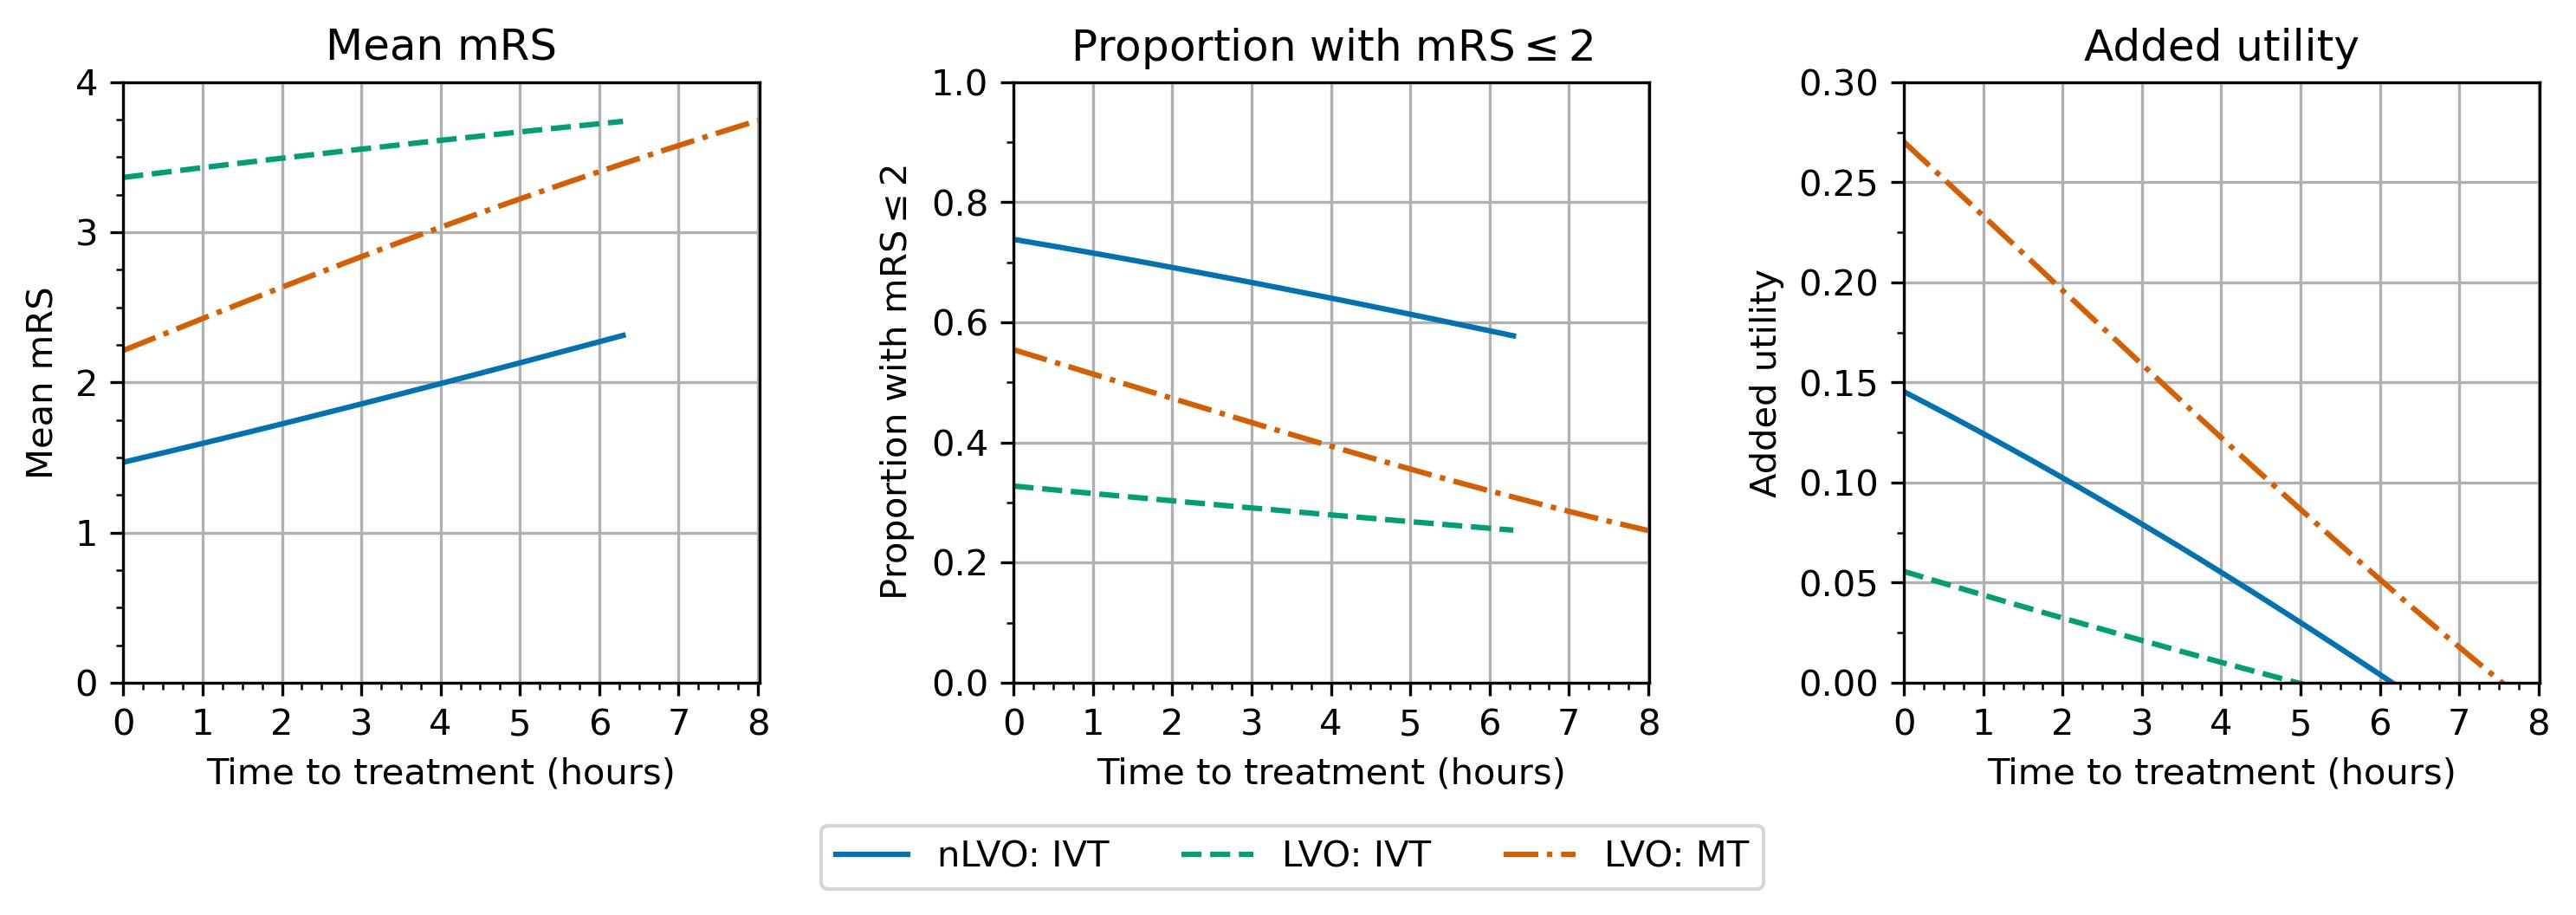
\includegraphics[width=1.0\textwidth]{./images/time_to_treatment}
\caption{Alternative outcome measures by by time from onset to treatment. Left: mean mRS. Middle: Proportion of patients with mRS 0-2. Right: Added utility.}
\label{fig:added_utility_six_in_one}
\end{figure}


\begin{figure}
\centering
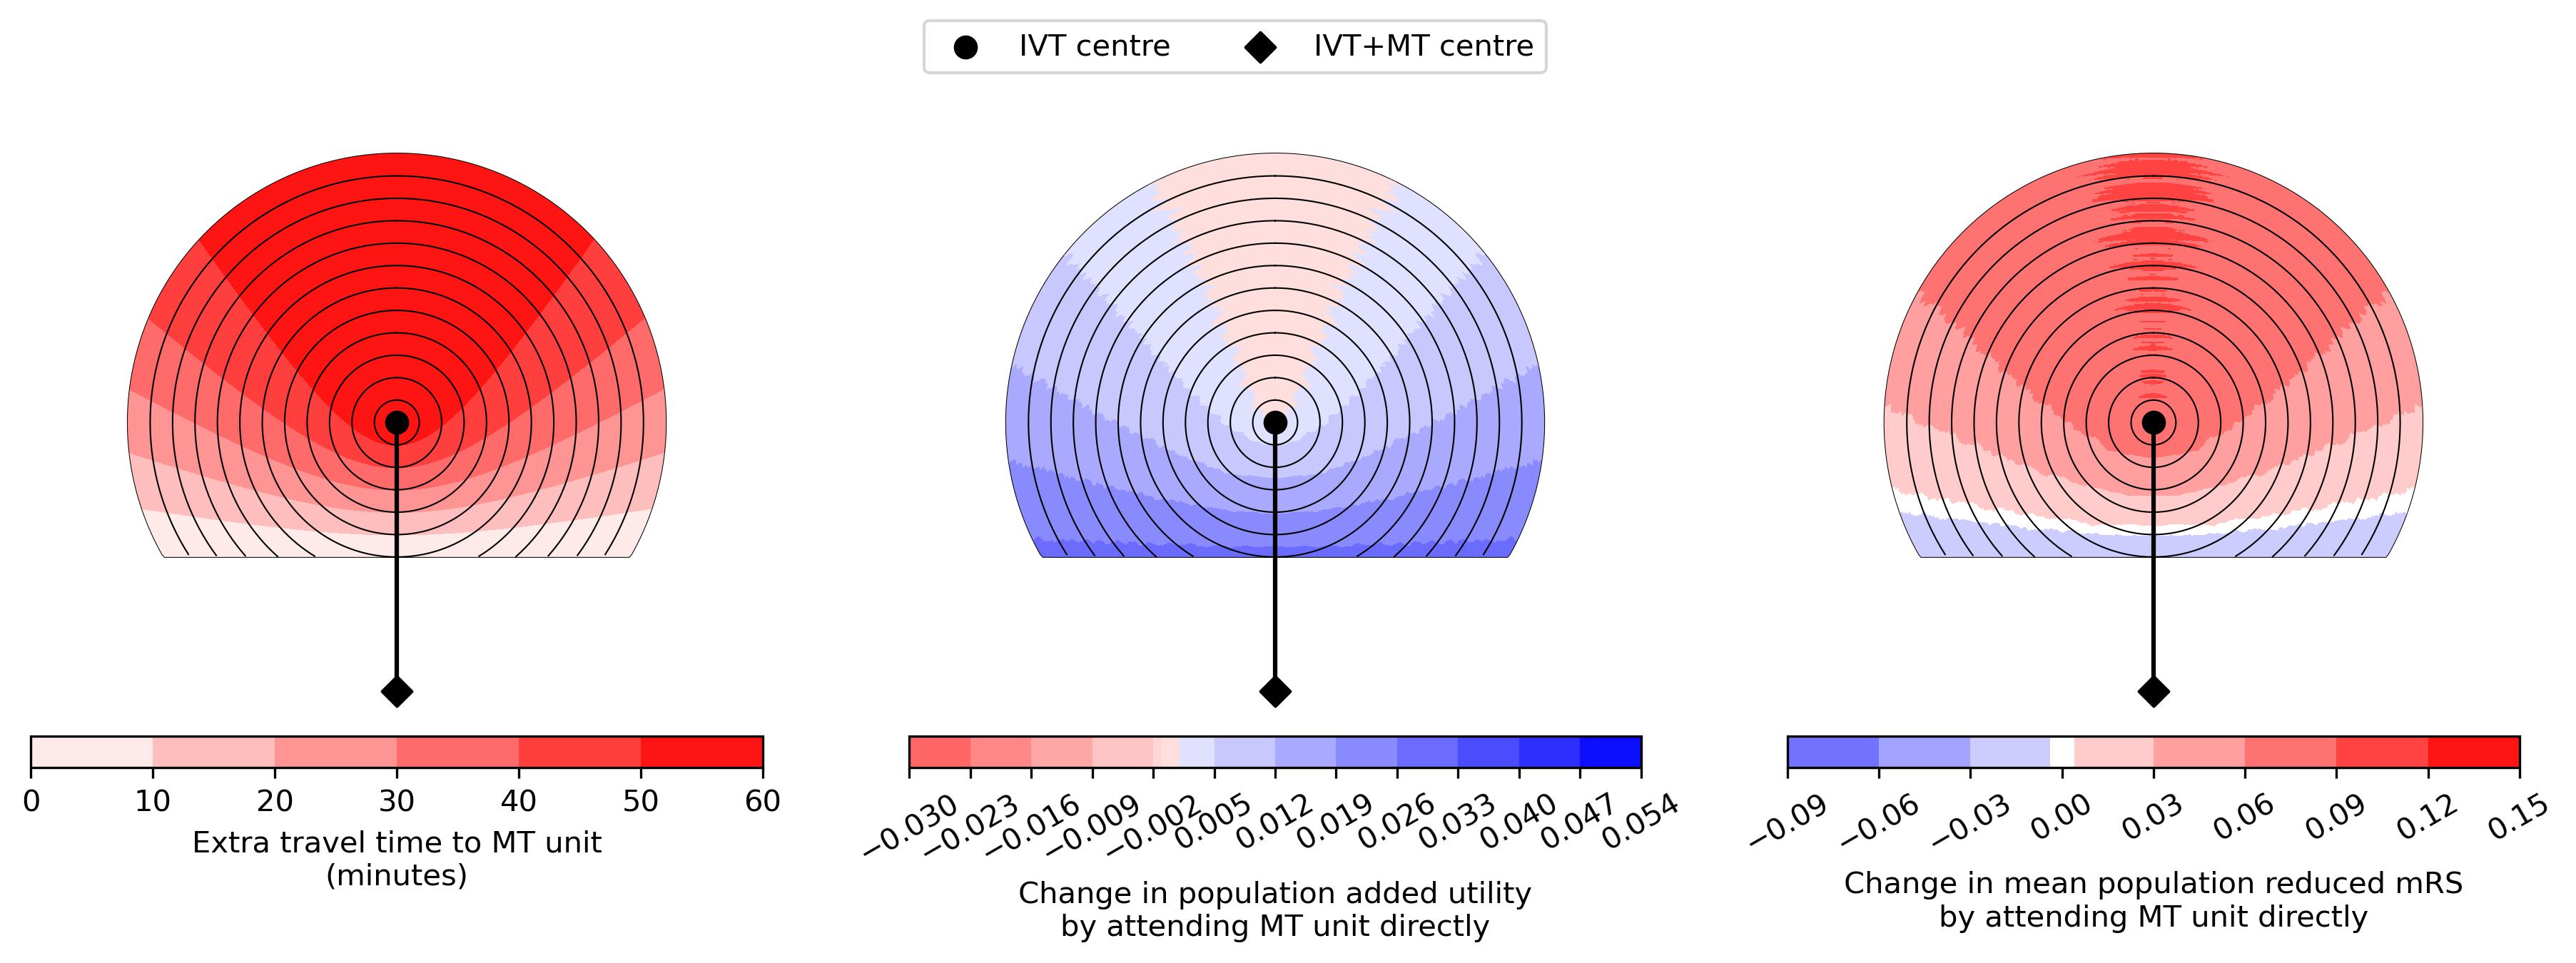
\includegraphics[width=1.0\textwidth]{./images/circle_plots_t-IVT-to-MT=60_t-onset-to-ambo=60}
\caption{The effect of bypassing an IVT-only unit in order to travel directly to a MT-capable unit that is 60 minutes away from the IVT-only unit. Results are for treatable patients (IVT and/or MT), with a mix of 35\% LVO and 65\% nLVO. An ambulance is assumed to arrive at the patient 60 minutes after stroke onset. Concentric circles represent 5 minutes travel time intervals from IVT-only unit. Left: Additional time required to attend the MT-capable unit  directly. Middle: Change in added utility by directly attending the MT-capable unit. Right: Change in population reduced average mRS by directly attending the MT-capable unit. Blue shades represent benefit, red shades represent disbenefit.}
\label{fig:added_utility_six_in_one}
\end{figure}

\begin{figure}
\centering
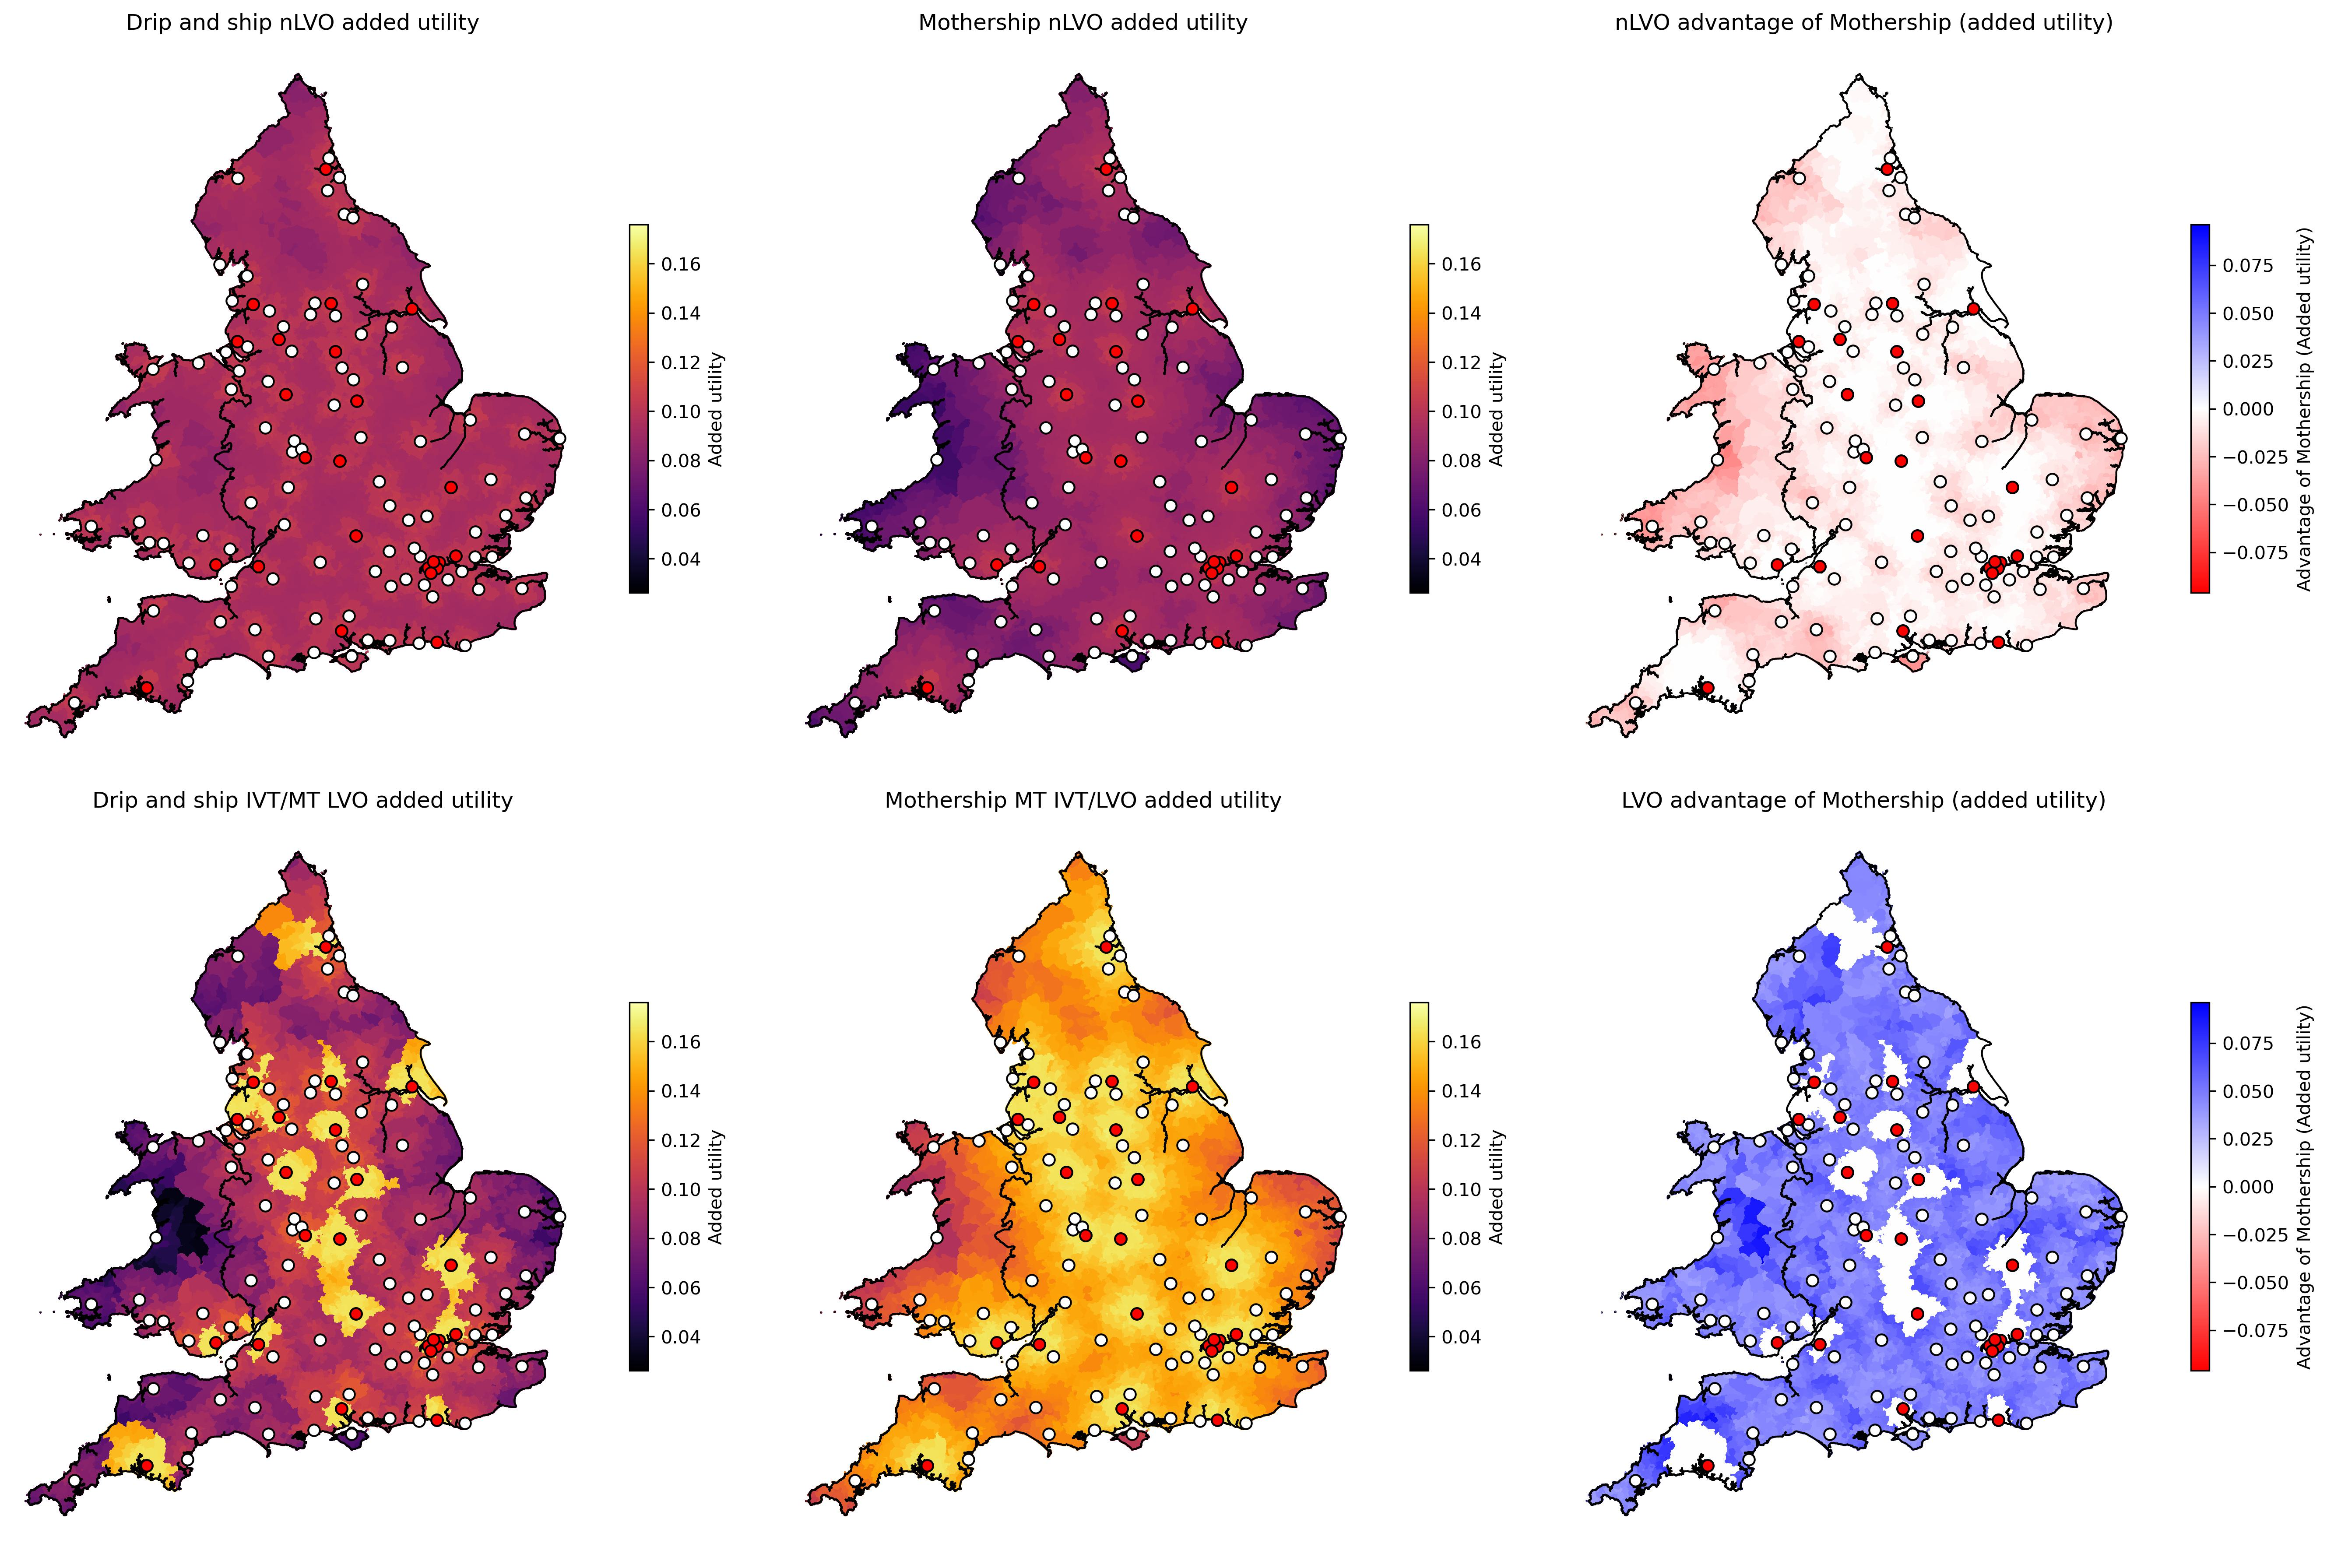
\includegraphics[width=1.0\textwidth]{./maps/added_utility_six_in_one}
\caption{Added utility from patients treated with IVT and/or MT. Top: nLVO treated with IVT. Bottom: LVO treated with IVT and/or MT. Left: Drip and ship. Middle: Mothership. Right: advantage of mothership over drip and ship. }
\label{fig:added_utility_six_in_one}
\end{figure}

\begin{figure}
\centering
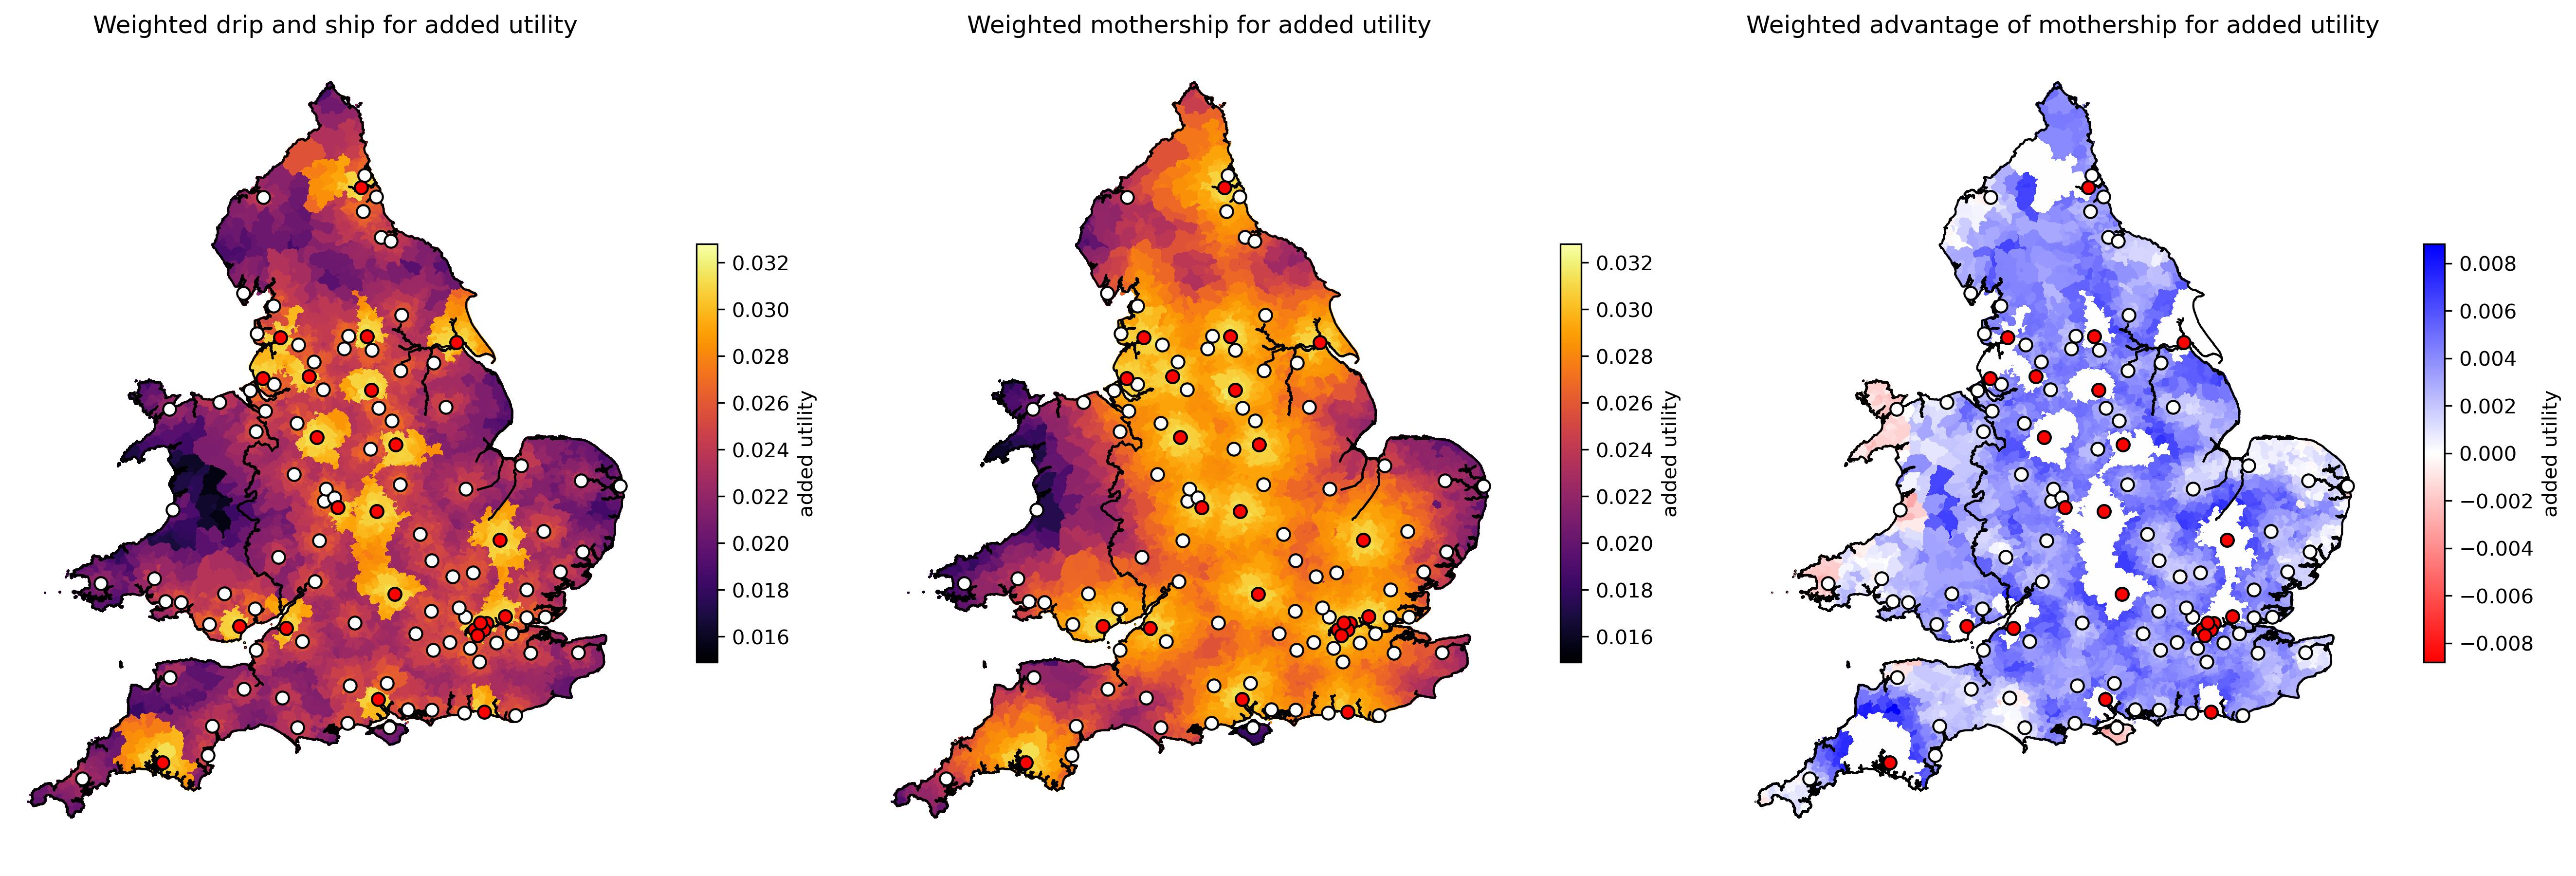
\includegraphics[width=1.0\textwidth]{./maps/added_utility_weighted_results}
\caption{Added utility }
\label{fig:added_utility_six_in_one}
\end{figure}

% Add reference section
\begin{multicols}{2}
\section{References}
\bibliographystyle{naturemag}
\bibliography{refs}
\end{multicols}

%TC:ignore
\section*{Appendix}

\appendix
\setcounter{section}{0}
\renewcommand{\thesection}{A\Alph{section}}
\setcounter{figure}{0}
\renewcommand{\thefigure}{A.\arabic{figure}}
\setcounter{table}{0}
\renewcommand{\thetable}{A.\arabic{table}}

\subsection{Modified Rankin Scale}

Modified Rankin Scale (mRS) is the most commonly used instrument to describe post-stroke functional outcome \citeappendix{quinn_functional_2009}. Table \ref{tab:mrs} shows a description of the seven level so f mRS along with utilties, from Wang \emph{et al.}\cite{wang_utility-weighted_2020}. Utilities are a measure of the preference or value that an individual or society gives a particular health state, with 1 being full health and 0 being dead (values of less than zero describe states where death is considered preferable).

\begin{minipage}{\textwidth}
\renewcommand*{\arraystretch}{1.5} % adjust row spacing
\begin{longtable}[]{@{}llr@{}}
\caption{A description of modified Rankin Scale score, with Utilities from Wang \emph{et al.}\cite{wang_utility-weighted_2020}}\\
\toprule
mRS & Description. & Utility\tabularnewline
\midrule
\endhead
0 & No symptoms. & 0.97\tabularnewline
1 & No significant disability: Able to carry out all usual activities,
despite some symptoms. & 0.88\tabularnewline
2 & \makecell[l]{Slight disability: Able to look after own affairs without assistance, but unable to carry \\ out all previous activities.} &
0.74\tabularnewline
3 & Moderate disability: Requires some help, but able to walk
unassisted. & 0.55\tabularnewline
4 & \makecell[l]{Moderately severe disability: Unable to attend to own bodily needs without assistance, \\ and unable to walk unassisted.} & 0.20\tabularnewline
5 & Severe disability: Requires constant nursing care and attention,
bedridden, incontinent. & -0.19\tabularnewline
6 & Dead. & 0.00\tabularnewline
\bottomrule
\label{app_tab:mrs}
\end{longtable}
\end{minipage}

\subsection{General model description}

% mRS distribution derivation

We define outcome in terms of probability distributions of mRS scores. 
\Anna{add description of mRS dists here}


% Probability with time:
% Words description:
We use these outcome probability distributions to model the variation of outcome probability with time for each combination of occlusion type and treatment.
% 
For a given mRS category $x$ at time $t$, the probability values, $P(\mRS\leq x\ |\ t)$, can be converted to odds, $O(\mRS\leq x\ |\ t)$, and \logodds, $\log_e[O(\mRS\leq x\ |\ t)]$, by using the standard definition $O=P/(1-P)$.
The \logodds\ can be modelled similarly to outcome \logoddsratio, which falls off approximately linearly with time\cite{emberson_effect_2014, fransen_time_2016}. 
% 
The known relation between \logodds\ and time can then be converted back into relations for odds and probability with time.

% Maths description:
We define a straight line fit $\log_e[O(\mRS\leq x\ |\ t)] = A_x + b_x t$
for constants $A_x$ and $b_x$ that differ for each mRS category $x$, $0\leq x \leq5$.
This gives an exponential form of odds where $O(\mRS\leq x\ |\ t) = \exp{(A_x + b_x t)}$.
The conversion to probability uses the inversion of the standard relation between probability and odds,  $P=O/(1+P)$. 
The final result is probability in the form of a logistic function:

\begin{equation}
P(\mRS\leq x\ |\ t) = \frac{1}{1+\exp{(A_x + b_x t)}}
\end{equation}


The constants $A_x$ and $b_x$ are found by considering the known data at $t=0$ and $t=\tne$. 
When $t=0$ then $A_x = \log_e[O(\mRS\leq x\ |\ t=0)]$ and when $t=\tne$ then $b_x = (\log_e[O(\mRS\leq x\ |\ t=\tne)] - A_x) / \tne$. 

The resulting distributions of probability with time are given in Figure~\ref{fig:app_probs_with_time} for each combination of occlusion type and treatment method.


\begin{figure}
    \centering
    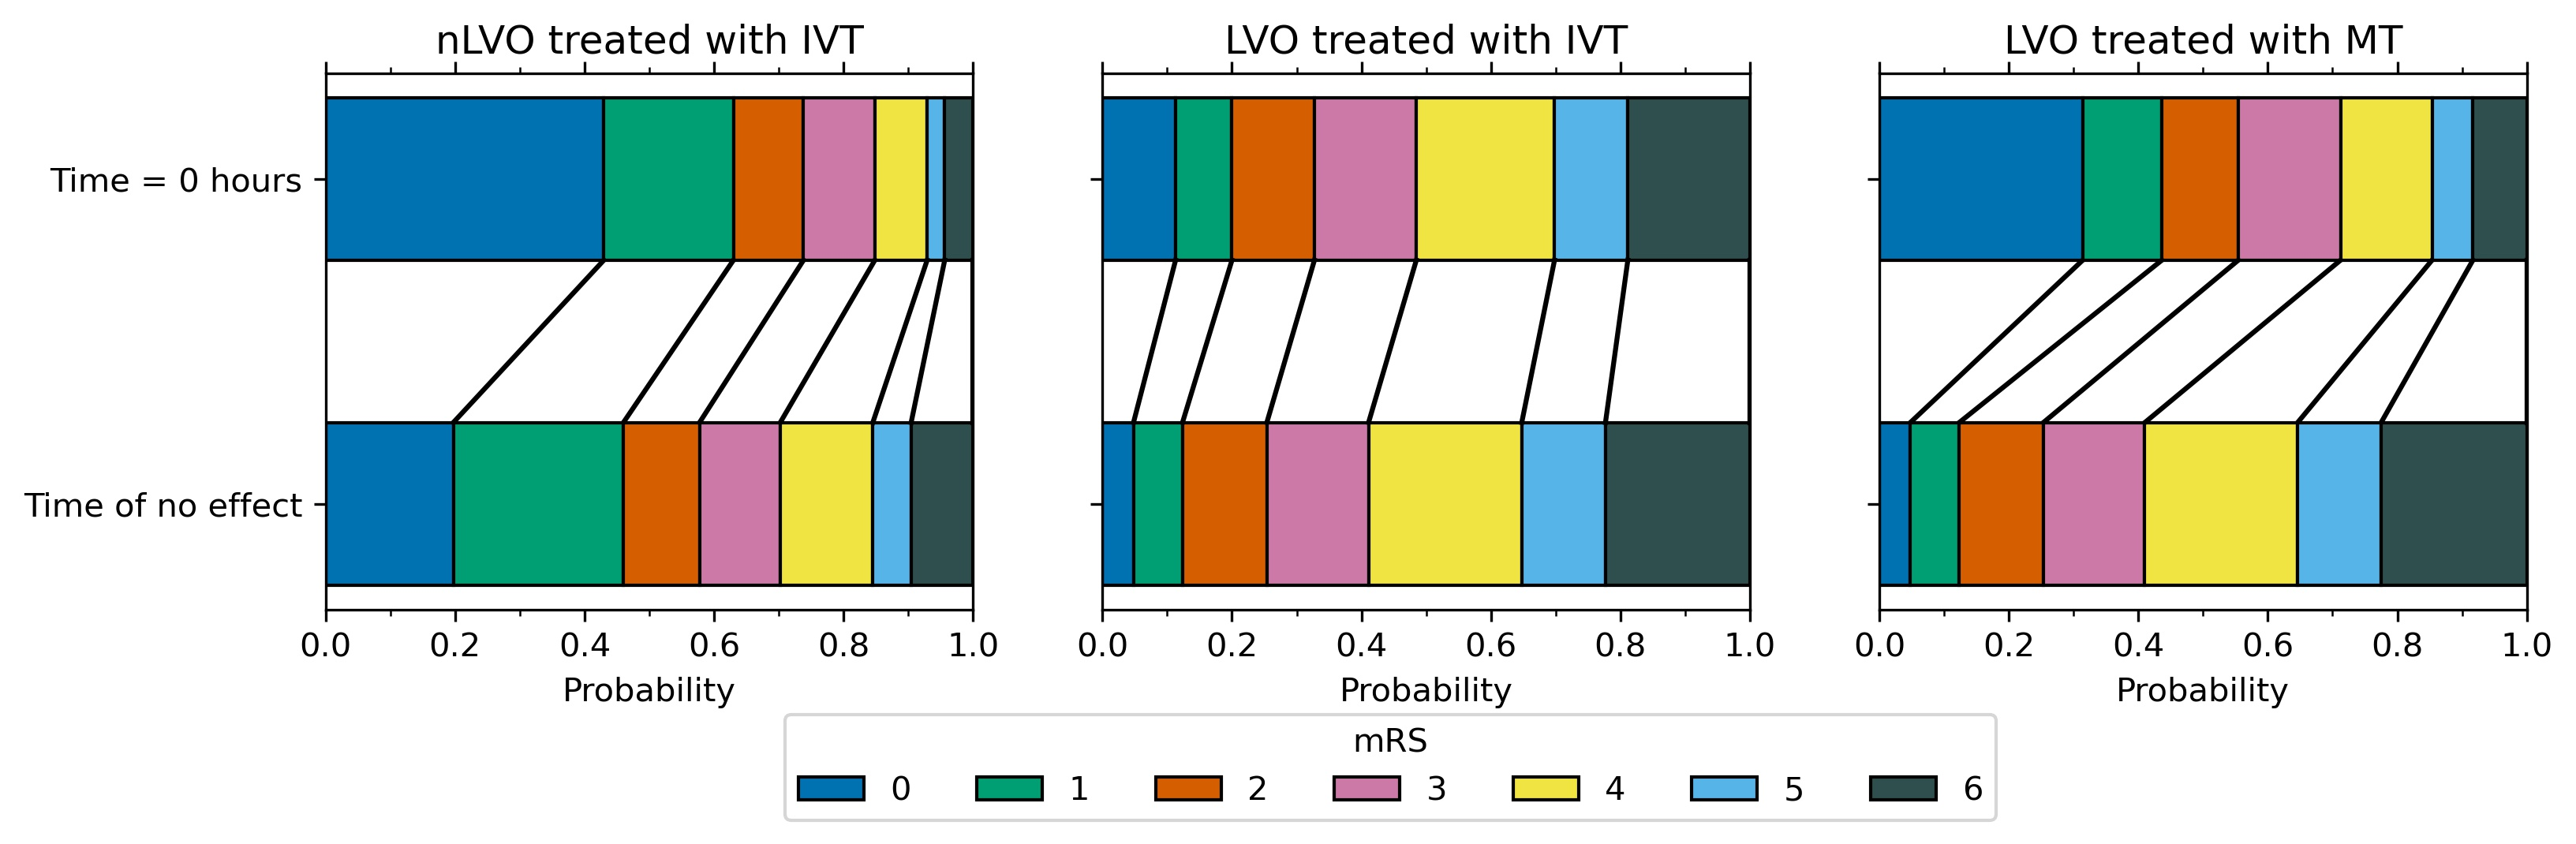
\includegraphics[width=\columnwidth]{images/dist_bars.jpg}
    \caption{
        The probability distributions of the mRS values of different patient populations. 
        The data sources and derivations \checkthis{are explained in the text...?}.
        The values associated with each distribution are tabulated in Table.... \checkthis{presumably? Or they can be plonked onto the figure.}}
    \label{app_fig:dist_bars}
\end{figure}

\begin{figure}
    \centering
    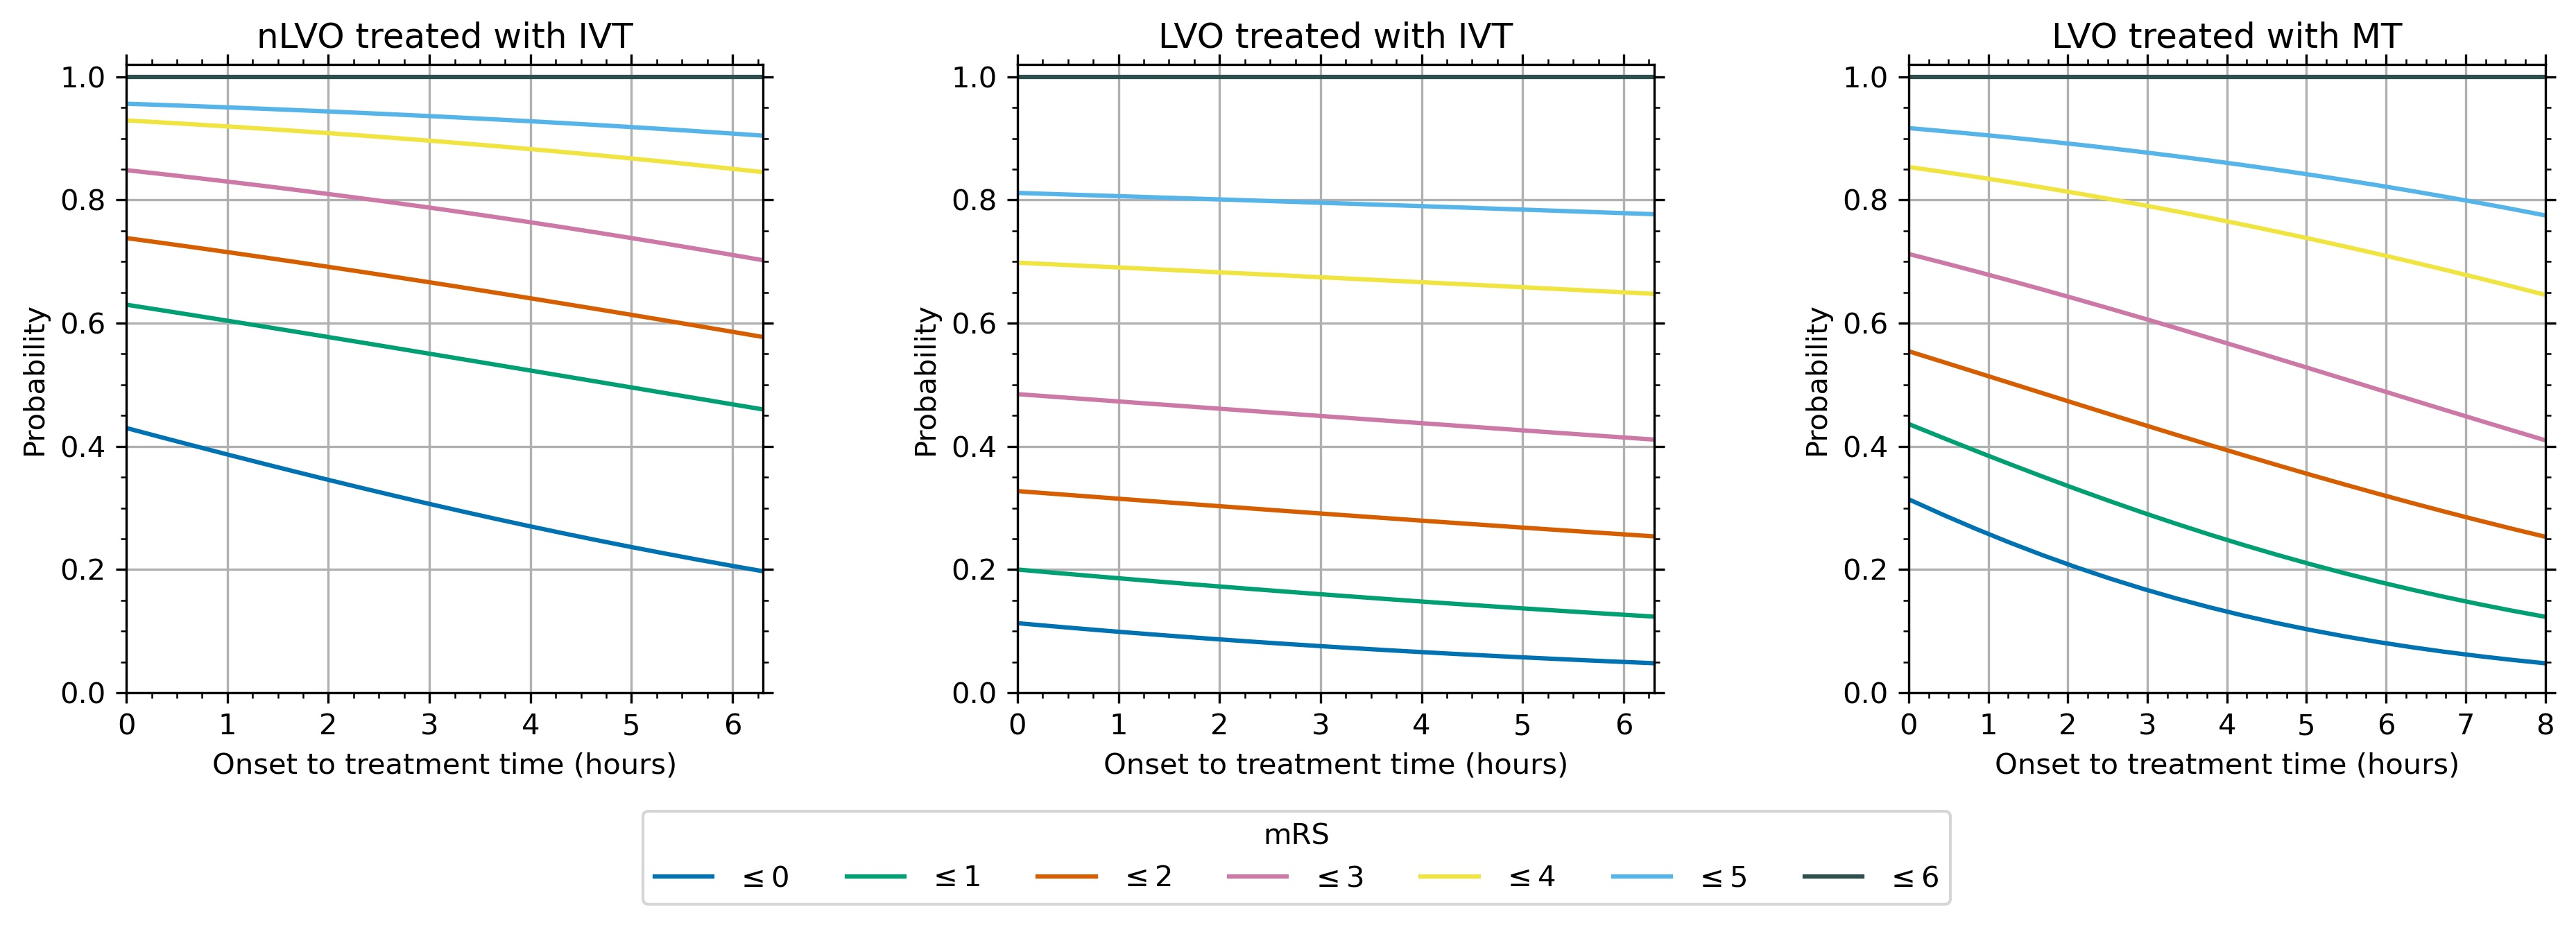
\includegraphics[width=\columnwidth]{images/probs_with_time.jpg}
    \caption{
        The variation of the mRS probability distributions with time.
        The maximum times shown are the times-of-no-effect, which for IVT is 6.3\,hr \cite{emberson_effect_2014},
        and for MT is 8.0\,hr\cite{goyal_endovascular_2016}\checkthis{check source}.
        }
    \label{fig:app_probs_with_time}
\end{figure}

\begin{figure}
    \centering
    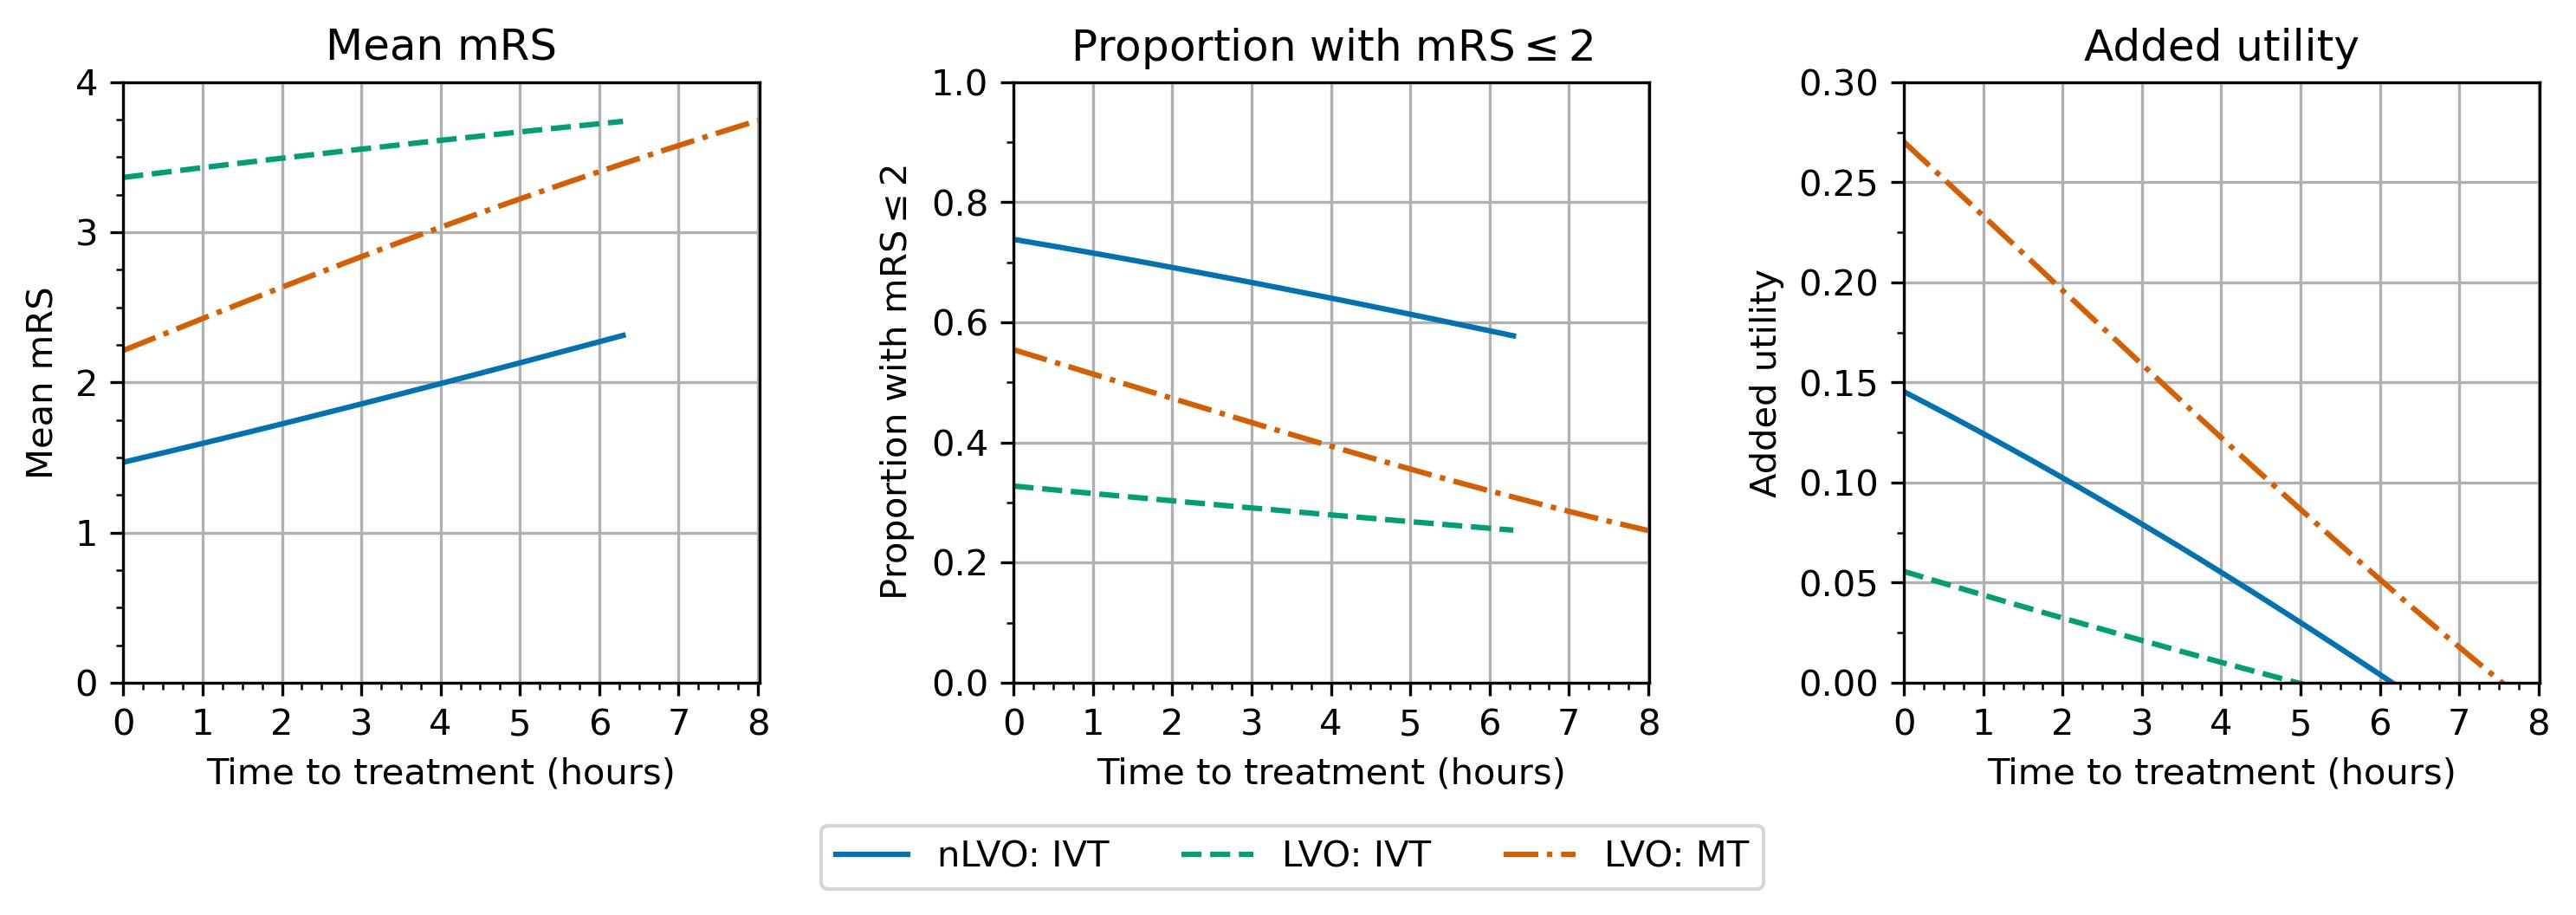
\includegraphics[width=\columnwidth]{images/time_to_treatment.jpg}
    \caption{
        The various outcomes for a representative patient population when the whole population has the same onset-to-treatment time and is given the treatment type. 
        \checkthis{should right-hand panel y-axis go below zero?}
        }
    \label{app_fig:changes_with_time}
\end{figure}


\begin{figure}
    \centering
    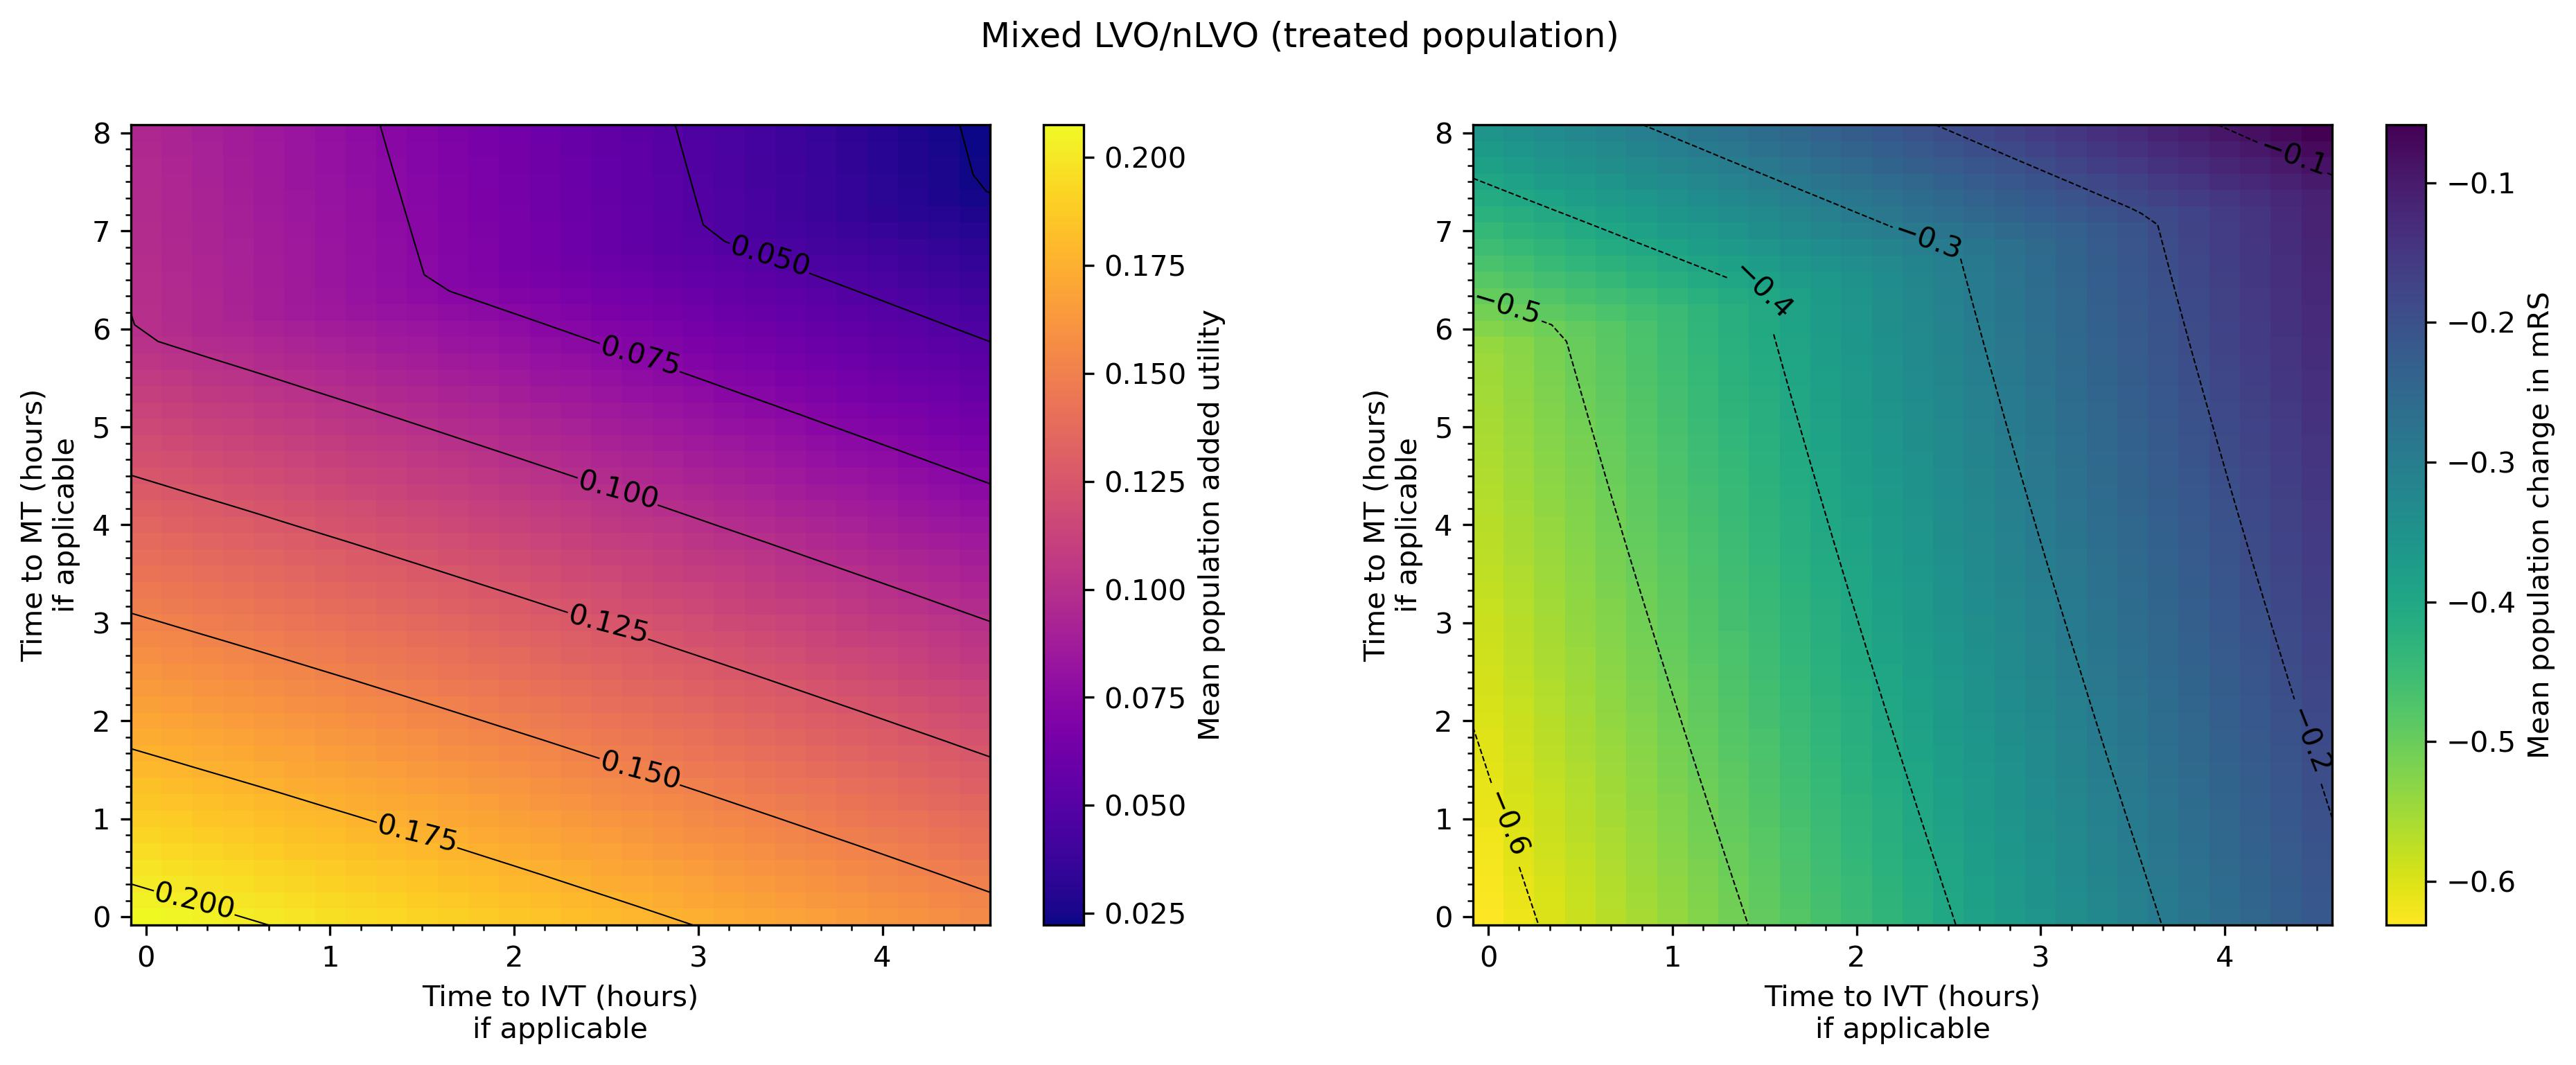
\includegraphics[width=\columnwidth]{images/matrix_utility_and_mRS.jpg}
    \caption{
        The expected mean change in utility (left panel) and mRS (right panel) for a representative patient population. At each combination of time to IVT and time to MT, every person in the population is given the treatments that they are eligible for. Larger resulting mean improvements are shown in paler colours.
        \checkthis{Why does the IVT time go up to 4.something hours when usually we use 6.3?}
        }
    \label{app_fig:matrix}
\end{figure}



%TC:endignore
\end{document}
